\documentclass[10pt]{article}
\usepackage[utf8]{inputenc}
\usepackage[T1]{fontenc}
\usepackage{amsmath}
\usepackage{amsfonts}
\usepackage{amssymb}
\usepackage[version=4]{mhchem}
\usepackage{stmaryrd}
\usepackage{bbold}
\usepackage{graphicx}
\usepackage[export]{adjustbox}
\graphicspath{ {./images/} }

\begin{document}
\section*{Diskrete und stetige Verteilungen}
\begin{center}
\begin{tabular}{|c|c|c|}
\hline
 & diskrete Zufallsvariablen & stetige Zufallsvariablen \\
\hline
Dichtefunktion / PDF/PMF & $f(x)=P(X=x)$ & $f(x)=F^{\prime}(x) \neq P(X=x)$ \\
\hline
\begin{tabular}{l}
Kumulative \\
Verteilungsfunktion / \\
CDF \\
\end{tabular} & $F(x)=P(X \leq x)=\sum_{u \leq x} f(u)$ & \( F(x)=P(X \leq x)=\int_{-\infty}^{x} f(u) d u \) \\
\hline
Wahrscheinlichkeiten & \( \begin{gathered} P(a \leq X \leq b)=\sum_{a \leq x \leq b} f(x) \\ P(a<X \leq b)=\sum_{a<x \leq b} f(x) \\ P(a<X<b)=\sum_{a<x<b} f(x) \\ P(a<X)=1-F(a) \end{gathered} \) & \( \begin{aligned} & \left.\begin{array}{l} P(a \leq X \leq b) \\ P(a<X \leq b) \\ P(a<X<b) \end{array}\right\}=\int_{a}^{b} f(x) d x \\ & \quad P(a<X)=1-F(a) \end{aligned} \) \\
\hline
\begin{tabular}{l}
Graphische \\
Darstellung von $f$ \\
\end{tabular} & Stabdiagramm & Graph \\
\hline
Erwartungwert & \( E(X)=\sum_{x \in \mathbb{R}} f(x) \cdot x \) & \( E(X)=\int_{-\infty}^{\infty} f(x) \cdot x d x \) \\
\hline
Varianz & \( V(X)=\sum_{x \in \mathbb{R}} f(x) \cdot(x-E(X))^{2} \) & \( V(X)=\int_{-\infty}^{\infty} f(x) \cdot(x-E(X))^{2} d x \) \\
\hline
\end{tabular}
\end{center}

\section*{Satz}
Für diskrete und stetige Zufallsvariablen $X$ und $Y$ gelten die folgenden Regeln:\\
(1) Linearität des Erwartungswertes:

$$
E(X+Y)=E(X)+E(Y) \text { und } E(\alpha X)=\alpha E(X) \text { mit } \alpha \in \mathbb{R}
$$

(2) Verschiebungssatz für die Varianz:

$$
V(X)=E\left(X^{2}\right)-(E(X))^{2}
$$

(3) $V(\alpha X+\beta)=\alpha^{2} \cdot V(X)$ mit $\alpha, \beta \in \mathbb{R}$.\\
(4) Sind $X$ und $Y$ stochastisch unabhängig, so gilt:

$$
V(X+Y)=V(X)+V(Y)
$$

\section*{Bemerkung}
Es ist effizienter, die Varianz mithilfe des Verschiebungssatzes zu berechnen als mithilfe der Definition.

\section*{Definition}
Eine diskrete Zufallsvariable $X$ heisst hypergeometrisch verteilt mit den Parametern $n$ (Anzahl Ziehungen ohne Zurücklegen), $N$ (Gesamtza aller Objekte) und $M$ (Gesamtzahl aller Merkmalsträger), wenn ihre Dichtefunktion (PMF) gegeben ist durch

$$
P(X=x)=\frac{\binom{M}{x} \cdot\binom{N-M}{n-x}}{\binom{N}{n}}
$$

Schreibweise: $X \sim H(N, M, n)$.\\
$X$ zählt, wie oft bei der $n$-fachen Ziehung (nacheinander und ohne Zurücklegen) ein Merkmalsträger gezogen wird.

\section*{Satz}
Für eine Zufallsvariable $X \sim H(N, M, n)$ gilt:\\
(1) $\mu=E(X)=n \cdot \frac{M}{N}$\\
(2) $\sigma^{2}=\mathrm{V}(X)=n \cdot \frac{M}{N} \cdot\left(1-\frac{M}{N}\right) \cdot \frac{N-n}{N-1}$\\
(3) $\sigma=S(X)=\sqrt{V(X)}$

\section*{Die Bernoulli Verteilung}
\section*{Definition}
Eine Zufallsvariable $X$ heisst Bernoulli-verteilt, wenn sie nur zwei verschiedene Werte annehmen kann: den Wert 1 mit der Wahrscheinlichke $P(X=1)=p$ und den Wert 0 mit der Wahrscheinlichkeit $P(X=0)=1-p$.

\section*{Satz}
Für Bernoulli-verteilte Zufallsvariablen $X$ gilt:\\
(1) $E(X)=E\left(X^{2}\right)=p$.\\
(2) $V(X)=p \cdot(1-p)$

\section*{Die Binomialverteilung}
\section*{Definition}
Eine diskrete Zufallsvariable $X$ heisst binomialverteilt mit den Parametern $n$ (Anzahl Wiederholungen) und $p$ (Wahrscheinlichkeit für ein Ergebnis 1), wenn ihre Dichtefunktion (PMF) gegeben ist durch

$$
P(X=x)=\binom{n}{x} \cdot p^{x} \cdot(1-p)^{n-x}
$$

Schreibweise: $X \sim B(n ; p)$.\\
$X$ zählt, wie oft bei der $n$-fachen Wiederholung eines Bernoulli-Experiments das Ergebnis 1 eintritt. Die Wahrscheinlichkeit für das Ergebnis wird üblicherweise mit $q=1-p$ bezeichnet.

Die $B(n ; p)$-verteilte Zufallsvariable $X$ kann als Summe von $n$ Bernoulli-verteilten Zufallsvariablen $X_{i}$ aufgefasst werden: $X=\sum_{i=1}^{n} X_{i}$. Dabei hält $X_{i}$ das Ergebnis des $i$-ten Experiments fest, und es gilt: $P\left(X_{i}=1\right)=p$.

\section*{Satz}
Für eine Zufallsvariable $X \sim B(n ; p)$ gilt:\\
(1) $\mu=E(X)=n p$\\
(2) $\sigma^{2}=\mathrm{V}(X)=n p q$\\
(3) $\sigma=S(X)=\sqrt{n p q}$

\section*{Faustregel zur Approximation}
Wenn die Bedingung $n \leq \frac{N}{20}$ erfüllt ist, kann die hypergeometrische Verteilung $H(N, M, n)$ gut durch die Binomialverteilung $B\left(n, \frac{M}{N}\right)$ angenähert werden: $H(N, M, n) \approx B\left(n, \frac{M}{N}\right)$

\section*{Die Poisson Verteilung}
\section*{Definition}
Eine diskrete Zufallsvariable $X$ heisst poissonverteilt mit dem Parameter $\lambda>0$ (durchschnittliche Anzahl Ereignisse pro betrachtetes Zeitintervall), wenn ihre Dichtefunktion (PMF) gegeben ist durch

$$
P(X=x)=e^{-\lambda} \cdot \frac{\lambda^{x}}{x!}
$$

Schreibweise: $X \sim \operatorname{Poi}(\lambda)$.\\
$X$ zählt die Anzahl der (stochastisch unabhängigen, gleichartigen) Ereignisse in einem betrachteten Zeitintervall.

\section*{Satz}
Für eine Zufallsvariable $X \sim \operatorname{Poi}(\lambda)$ gilt:\\
(1) $\mu=E(X)=\lambda$\\
(2) $\sigma^{2}=\mathrm{V}(X)=\lambda$\\
(3) $\sigma=S(X)=\sqrt{\lambda}$

\section*{Faustregel zur Approximation}
Wenn die Bedingung $n \geq 50$ und $p \leq 0.1$ erfüllt ist, kann die Binomialverteilung $B(n, p)$ gut durch die Poissonverteilung Poi $(n \cdot p)$ angenähert werden: $B(n, p) \approx \operatorname{Poi}(n \cdot p)$.

\section*{Gauss'sche Normalverteilung}
\section*{Definition}
Eine stetige Zufallsvariable $X$ heisst normalverteilt mit den Parametern $\mu, \sigma \in \mathbb{R}, \sigma>0$, wenn sie folgende Dichtefunktion (PDF) hat:

$$
\varphi_{\mu, \sigma}(x)=\frac{1}{\sqrt{2 \pi} \cdot \sigma} \cdot e^{-\frac{1}{2}\left(\frac{x-\mu}{\sigma}\right)^{2}}
$$

Schreibweise: $X \sim N(\mu ; \sigma)$\\
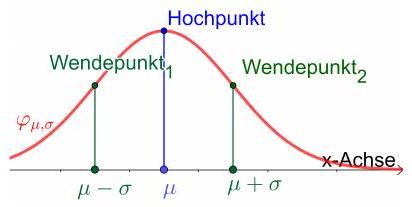
\includegraphics[width=\linewidth]{images/2025_01_02_c6e65a99bfeab7c89599g-3(1)}

Die kumulative Verteilungsfunktion (CDF) von $\varphi_{\mu, \sigma}(x)$ wird mit $\phi_{\mu, \sigma}(x)$ bezeichnet. Sie ist definiert durch:

$$
\phi_{\mu, \sigma}(x)=P(X \leq x)=\int_{-\infty}^{x} \varphi_{\mu, \sigma}(t) d t=\frac{1}{\sqrt{2 \pi} \cdot \sigma} \cdot \int_{-\infty}^{x} e^{-\frac{1}{2}\left(\frac{t-\mu}{\sigma}\right)^{2}} d t
$$

\begin{center}
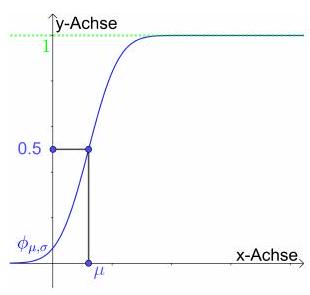
\includegraphics[width=\linewidth]{2025_01_02_c6e65a99bfeab7c89599g-3}
\end{center}

Ist $\mu=0$ und $\sigma=1$, so spricht man von der Standardnormalverteilung. Ihre Dichtefunktion (PDF) wird mit $\varphi$ bezeichnet; sie ist gegeben du

$$
\varphi(x)=\frac{1}{\sqrt{2 \pi}} \cdot e^{-\frac{1}{2} x^{2}}
$$

Ihre Verteilungsfunktion (CDF) $\phi_{0,1}(x)$ wird mit $\phi(x)$ bezeichnet. Schreibweise: $X \sim N(0 ; 1)$.\\
Die Verteilungsfunktion der Normalverteilung kann nicht auf elementare Weise berechnet werden. Für inre Werte gibt es Tabellen (Papula 12 Aufl. S. 514); die Tabellen beziehen sich allerdings immer auf die Standardnormalverteilung.

\section*{Bemerkung}
Die Dichtefunktion (PDF) $\varphi_{\mu, \sigma}(x)$ hat folgende Eigenschaften:\\
(a) Sie ist symmetrisch bezüglich der Geraden $x=\mu$.\\
(b) Sie hat Wendepunkte an den Stellen $\mu-\sigma$ und $\mu+\sigma$.\\
(c) Sie ist normiert, d.h. es gilt:\\
$\int_{-\infty}^{\infty} \varphi_{\mu, \sigma}(x) d x=\frac{1}{\sqrt{2 \pi} \cdot \sigma} \cdot \int_{-\infty}^{\infty} e^{-\frac{1}{2}\left(\frac{x-\mu}{\sigma}\right)^{2}} d x=1$\\
(d) Eine Änderung von $\mu$ bewirkt eine Verschiebung in $x$-Richtung; je grösser $\sigma$ ist, desto breiter und niedriger wird die Glockenkurve.\\
(e) Für eine Zufallsvariable $X \sim N(\mu ; \sigma)$ gilt: $E(X)=\mu$ und $V(X)=\sigma^{2}$.

\section*{Bemerkung}
Bei einer Zufallsvariable $X$, die der Normalverteilung $N(\mu ; \sigma)$ folgt, liegen

\begin{itemize}
  \item ca. $68 \%$ der beobachteten Werte zwischen $\mu-\sigma$ und $\mu+\sigma$,
  \item ca. $95 \%$ der beobachteten Werte zwischen $\mu-2 \sigma$ und $\mu+2 \sigma$,
  \item ca. $99.7 \%$ der beobachteten Werte zwischen $\mu-3 \sigma$ und $\mu+3 \sigma$.\\
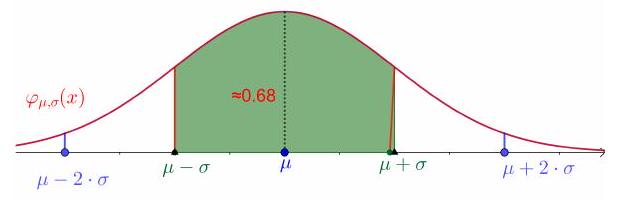
\includegraphics[width=\linewidth]{images/2025_01_02_c6e65a99bfeab7c89599g-4}
\end{itemize}

Wichtige Eigenschaften einer $N(\mu ; \sigma)$-verteilten Zufallsvariable $X$

$$
\begin{aligned}
& \phi_{\mu, \sigma}^{\prime}(x)=\varphi_{\mu, \sigma}(x) \\
& \begin{aligned}
\phi_{\mu, \sigma}(x)=\phi\left(\frac{x-\mu}{\sigma}\right) \\
\begin{aligned}
P(a \leq X \leq b) & =\phi_{\mu, \sigma}(b)-\phi_{\mu, \sigma}(a) \\
P(|X-\mu| \leq \varepsilon) & =P(\mu-\varepsilon \leq X \leq \mu+\varepsilon) \\
& =2 \cdot \phi_{\mu, \sigma}(\mu+\varepsilon)-1 \\
& =1-2 \cdot \phi_{\mu, \sigma}(\mu-\varepsilon)
\end{aligned}
\end{aligned} \begin{aligned}
\end{aligned} \\
&
\end{aligned}
$$

In den Aussagen können $\leq$ Zeichen nach Belieben durch $<$ Zeichen ersetzt werden.

\section*{Zentraler Grenzwertsatz}
Gegeben sind lauter identisch verteilte und stochastisch unabhängige Zufallsvariablen $X_{1}, X_{2}, \ldots$, alle mit demselben Erwartungswert $\mu$ und derselben Varianz $\sigma^{2}$. Dann hat die Summe

$$
S_{n}=\sum_{i=1}^{n} X_{i}
$$

den Erwartungswert $n \mu$ und die Varianz $n \sigma^{2}$ und ist annähernd $N(n \mu ; \sqrt{n} \sigma)$ verteilt.

Das arithmetische Mittel

$$
\bar{X}_{n}=S_{n} / n
$$

hat den Erwartungswert $\mu$ und die Varianz $\sigma^{2} / n$ und ist annähernd $N\left(\mu ; \frac{\sigma}{\sqrt{n}}\right)$ verteilt.

Die Verteilungsfunktion (CDF) $F_{n}(u)$ der dazugehörigen standardisierten\\
Zufallsvariablen

$$
U_{n}=\frac{S_{n}-n \mu}{\sqrt{n} \sigma}=\frac{\bar{X}_{n}-\mu}{\sigma / \sqrt{n}}
$$

konvergiert für $n \rightarrow \infty$ gegen die Verteilungsfunktion $\phi(u)$ der\\
Standardnormalverteilung:

$$
\lim _{n \rightarrow \infty} F_{n}(u)=\phi(u)=\frac{1}{\sqrt{2 \pi}} \cdot \int_{-\infty}^{u} e^{-\frac{1}{2} t^{2}} d t
$$

Zuletzt geändert: Montag, 20. September 2021, 17:21

4 4. Zusammenfassung: Elementare Wahrscheinlichkeitsrechnung

\section*{Direkt zu:}

\end{document}